%
% This is a borrowed LaTeX template file for lecture notes for CS267,
% Applications of Parallel Computing, UCBerkeley EECS Department.
% Now being used for CMU's 10725 Fall 2012 Optimization course
% taught by Geoff Gordon and Ryan Tibshirani.  When preparing 
% LaTeX notes for this class, please use this template.
%
% To familiarize yourself with this template, the body contains
% some examples of its use.  Look them over.  Then you can
% run LaTeX on this file.  After you have LaTeXed this file then
% you can look over the result either by printing it out with
% dvips or using xdvi. "pdflatex template.tex" should also work.
%
\documentclass[twoside]{article}
\usepackage{graphicx}
\usepackage{tikz}
\usepackage{mathpazo}
\usetikzlibrary{decorations.pathmorphing}


\setlength{\oddsidemargin}{0.25 in}
\setlength{\evensidemargin}{-0.25 in}
\setlength{\topmargin}{-0.6 in}
\setlength{\textwidth}{6.5 in}
\setlength{\textheight}{8.5 in}
\setlength{\headsep}{0.75 in}
\setlength{\parindent}{0 in}
\setlength{\parskip}{0.1 in}
%
% ADD PACKAGES here:
%
\usepackage{amsmath,amsfonts,graphicx}
%
% The following commands set up the lecnum (lecture number)
% counter and make various numbering schemes work relative
% to the lecture number.
%
\newcounter{lecnum}
\renewcommand{\thepage}{\thelecnum-\arabic{page}}
\renewcommand{\thesection}{\thelecnum.\arabic{section}}
\renewcommand{\theequation}{\thelecnum.\arabic{equation}}
\renewcommand{\thefigure}{\thelecnum.\arabic{figure}}
\renewcommand{\thetable}{\thelecnum.\arabic{table}}
%
% The following macro is used to generate the header.
%
\newcommand{\lecture}[5]{
   \pagestyle{myheadings}
   \thispagestyle{plain}
   \newpage
   \setcounter{lecnum}{#1}
   \setcounter{page}{1}
   \noindent
   \begin{center}
   \framebox{
      \vbox{\vspace{2mm}
    \hbox to 6.28in { {\bf Physics 467/667: Thermodynamics/Statistical Physics
	\hfill Spring 2017} }
       \vspace{4mm}
       \hbox to 6.28in { {\Large \hfill Lecture #1: #2  \hfill} }
       \vspace{2mm}
       \hbox to 6.28in { {\it Lecturer: #3 \hfill Scribes: #4} }
      \vspace{2mm}}
   }
   \end{center}
   \markboth{Lecture #1: #2}{Lecture #1: #2}
   \vspace*{4mm}
}
%
%
% Convention for citations is authors' initials followed by the year.
% For example, to cite a paper by Leighton and Maggs you would type
% \cite{LM89}, and to cite a paper by Strassen you would type \cite{S69}.
% (To avoid bibliography problems, for now we redefine the \cite command.)
% Also commands that create a suitable format for the reference list.
\renewcommand{\cite}[1]{[#1]}
\def\beginrefs{\begin{list}%
        {[\arabic{equation}]}{\usecounter{equation}
         \setlength{\leftmargin}{2.0truecm}\setlength{\labelsep}{0.4truecm}%
         \setlength{\labelwidth}{1.6truecm}}}
\def\endrefs{\end{list}}
\def\bibentry#1{\item[\hbox{[#1]}]}
%Use this command for a figure; it puts a figure in wherever you want it.
%usage: \fig{NUMBER}{SPACE-IN-INCHES}{CAPTION}
\newcommand{\fig}[3]{
			\vspace{#2}
			\begin{center}
			Figure \thelecnum.#1:~#3
			\end{center}
	}
% Use these for theorems, lemmas, proofs, etc.
\newtheorem{theorem}{Theorem}[lecnum]
\newtheorem{lemma}[theorem]{Lemma}
\newtheorem{proposition}[theorem]{Proposition}
\newtheorem{claim}[theorem]{Claim}
\newtheorem{corollary}[theorem]{Corollary}
\newtheorem{definition}[theorem]{Definition}
\newenvironment{proof}{{\bf Proof:}}{\hfill\rule{2mm}{2mm}}
% **** IF YOU WANT TO DEFINE ADDITIONAL MACROS FOR YOURSELF, PUT THEM HERE:
\newcommand\E{\mathbb{E}}
\begin{document}
%FILL IN THE RIGHT INFO.
%\lecture{**LECTURE-NUMBER**}{**DATE**}{**LECTURER**}{**SCRIBE**}
\lecture{10}{Entropy and Heat}{Qiang Zhu}{scribe-name1,2,3}
%\footnotetext{These notes are partially based on those of Nigel Mansell.}
% **** YOUR NOTES GO HERE:
% Some general latex examples and examples making use of the
% macros follow.  
%**** IN GENERAL, BE BRIEF. LONG SCRIBE NOTES, NO MATTER HOW WELL WRITTEN,
%**** ARE NEVER READ BY ANYBODY.

\section{Some useful equations} % Don't be this informal in your notes!
\begin{equation} \label{idealgas} PV = nRT = NkT \end{equation}
\begin{equation} \label{Avogadro} N = n \times N_A \end{equation}
\begin{equation} \label{PV-micro} PV = Nm{\overline v_x^2} = NkT\end{equation}
\begin{equation} \label{eqpartition} U_{thermal} = N \cdot f \cdot \frac{1}{2}kT \end{equation}
\begin{equation} \label{1stlaw} \Delta{U} = Q + W \end{equation}
\begin{equation} \label{work3} \Delta W = - P \Delta{V} \end{equation}
\begin{equation} \label{entropy} S = k \text{ln}\Omega \end{equation}
\begin{equation} \label{pentropy} T = \frac {\partial{U}} {\partial{S}} \end{equation}

\section{Mechanical Equilibrium and Pressure}
In the last lecture, we just learned the relation between $S$ and $T$, is there any analogy between $S$ and $P$.

\begin{figure}[h]
\centering
\begin{tikzpicture}[thick]
\draw (0,0.4) -- (8,0.4) -- (8,4) -- (0,4) -- (0,0.4);
\draw (0.2,0.6) -- (4.4,0.6) -- (4.4,3.8) -- (0.2,3.8) -- (0.2,0.6);
\node at (1.8,2.8) {$U_A, V_A, S_A$};
\node at (1.8,2.2) {$P_A$};
\draw (7.8,0.6) -- (4.6,0.6) -- (4.6,3.8) -- (7.8,3.8) -- (7.8,0.6);
\node at (6.0,2.8) {$U_B, V_B, S_B$};
\node at (6.0,2.2) {$P_B$};
\draw [->,decorate,decoration=snake] (3.6,2) -- (5.0,2) node [above, xshift=-0.8cm]{pressure flow};
\end{tikzpicture}
\caption{A schematic pressure flow between two gases.}
\end{figure}

Again, we start from the condition when the system reaches its equilibrium,
\begin{equation} \label{entropy} 
\frac {\partial{S_\text{total}}} {\partial{U_A}}=0     ~~~~~~~~ \rightarrow~~~~~~~~  \frac {\partial{S_\text{total}}} {\partial{V_A}}=0
\end{equation}
as, $S$ is the function of $U$ and $V$.

We already applied the 1st condition in the previous lecture. How about the 2nd condition? 
\begin{equation} \label{entropy} 
\frac {\partial{S_A}} {\partial{V_A}} +  \frac {\partial{V_B}} {\partial{V_A}} =0     ~~~~~~~~ \rightarrow~~~~~~~~  
\frac {\partial{S_A}} {\partial{V_A}} =  \frac {\partial{V_B}} {\partial{V_B}} 
\end{equation}

What's the physical meaning of $\partial{S_A}/\partial{V_A}$? \\
If we dig a bit on the units, we will find $\partial{S_A}/\partial{V_A}$ has a unit of N$\cdot$m/K, about $P/T$ hence we guess
\begin{equation} \label{entropy} 
\frac {P}{T} =  (\frac {\partial{S}} {\partial{V}})_{U,N}     ~~~~~~~~ \rightarrow~~~~~~~~  
P = T (\frac {\partial{S}} {\partial{V}})_{U,N}
\end{equation}

Recall that we know how to calculate $S$,
\begin{equation} S = Nk\text{ln}V + 3/2Nk\text{ln}U - Nk\text{ln}(f(N)) \end{equation}
\begin{equation} P = T(\frac {\partial{S}} {\partial{V}})  = \frac{NKT}{V}\end{equation}
\begin{equation} PV = NkT \end{equation}
Again, we proved the ideal gas law.

\section{Thermodynamic Identity}
From the above sections, it seems that $\Delta{S}$ can be divided into two parts, 
\begin{enumerate}
\item $\Delta{U}$, to account for the heat flow
\item $\Delta{V}$, to account for the pressure flow
\end{enumerate}

Let's say,
\begin{equation} \Delta{S} = (\frac {\Delta{S}}{\Delta{U}})\Delta{U} + (\frac {\Delta{S}}{\Delta{V}})\Delta{V}  \end{equation}
Suppose each step is very small, we use 
\begin{equation} dS = (\frac{\partial S}{\partial U})dU + (\frac{\partial S}{\partial V})dV  \end{equation}
\begin{equation} dS = \frac{dU}{T} + (\frac{PdV}{T}  \end{equation}
\begin{equation} TdS = dU + PdV  \end{equation}
\begin{equation} dU = TdS - PdV  \end{equation}
This is {\bf Thermodynamic Identity}
If you compare it with the 1st law, it just substitute $TdS$ as $Q$, which is actually the old definition of entropy.
\begin{enumerate}
\item $\Delta{U}=0$, $dU=TdS$
\item $\Delta{V}=0$, $TdS=PdV$
\end{enumerate}

{\bf Exercise}
Under constant entropy
\begin{equation} (\frac{\partial S}{\partial U})dU + (\frac{\partial S}{\partial V})dV = 0 \end{equation}
\begin{equation} dU = -PdV \end{equation}
isentropic = quasistatic + adibatic \\
\begin{equation} \Delta{S} = S_f-S_i = \int^{T_f}_{T_i} \frac{C_P}{T} dT \end{equation}
$S(300K)$ = $S(0K) + C_P \int^{300}_{0} \frac{1}{T} dT$ = 5.8 + 3.5*8.31*ln(300) = 173.89 J/K.\\
This value looks much smaller than the reference value in the appendix (197.67 J/K), because of constant volume assumption is not realistic.
A more realistic solution is
\begin{equation} \Delta{S} = C_V\text{ln}\frac{P_B}{P_A} + C_P\text{ln}\frac{V_B}{V_A}\end{equation}
when you consider $Q = U-W$.

\begin{equation} \Delta{S} = \frac{Q}{T} ~~~~~~~~\text{quasistatic}\end{equation}
\begin{equation} \Delta{S} > \frac{Q}{T} ~~~~~~~~\text{in practice}\end{equation}

\begin{enumerate}
\item Very faster compression
\item free expansion
\end{enumerate}



\section{Homework}
Problem 3.27, 3.30, 3.31, 3.32, 3.33
\end{document}

